\documentclass{ctexart}
\usepackage{amsmath, mathrsfs, amsfonts}
\usepackage{tikz}
\usepackage{graphicx}
\usetikzlibrary{patterns}    % 绘制阴影区域需要加入的库

% library

\begin{document}

\begin{figure}[htp]
    \centering
    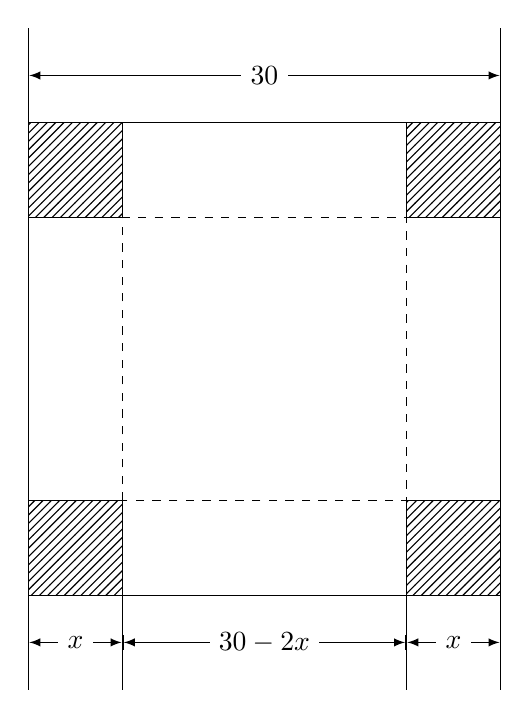
\begin{tikzpicture}[>=latex,scale=.6]
        \draw (0,0) rectangle (10,10);
        \draw[dashed] (2,2) rectangle (8,8);
        \draw[pattern=north east lines] (0,0) rectangle (2,2);    % 有的PDF阅读器渲染会存在一些差别
        \draw[pattern=north east lines] (8,0) rectangle (10,2);
        \draw[pattern=north east lines] (0,8) rectangle (2,10);
        \draw[pattern=north east lines] (8,8) rectangle (10,10);

        \foreach \x in {0,2,8,10}
        {
            \draw (\x,0)--(\x,-2);
        }
        \draw[|<->|] (2,-1)--node[fill=white]{$30-2x$}(8,-1);
        \draw (0,10)--(0,12);
        \draw (10,10)--(10,12);
        \draw[|<->|] (0,11)--node[fill=white]{$30$}(10,11);
        \draw[|<->|] (0,-1)--node[fill=white]{$x$}(2,-1);
        \draw[|<->|] (8,-1)--node[fill=white]{$x$}(10,-1);

    \end{tikzpicture}

    \caption{<caption>}
\end{figure}

\end{document}